\section{Auswertung}
\label{sec:Auswertung}

\subsection{Fouriesynthese}
Im ersten Teil des Experiments wurden wie in der Durchführung beschrieben die Spannungsverläufe zusammengesetzt. 

In Abbildung (\ref{fig:plot1}) ist die Fouriereihe der Sägezahnspannung zu sehen.
\begin{figure}[H]
  \centering
  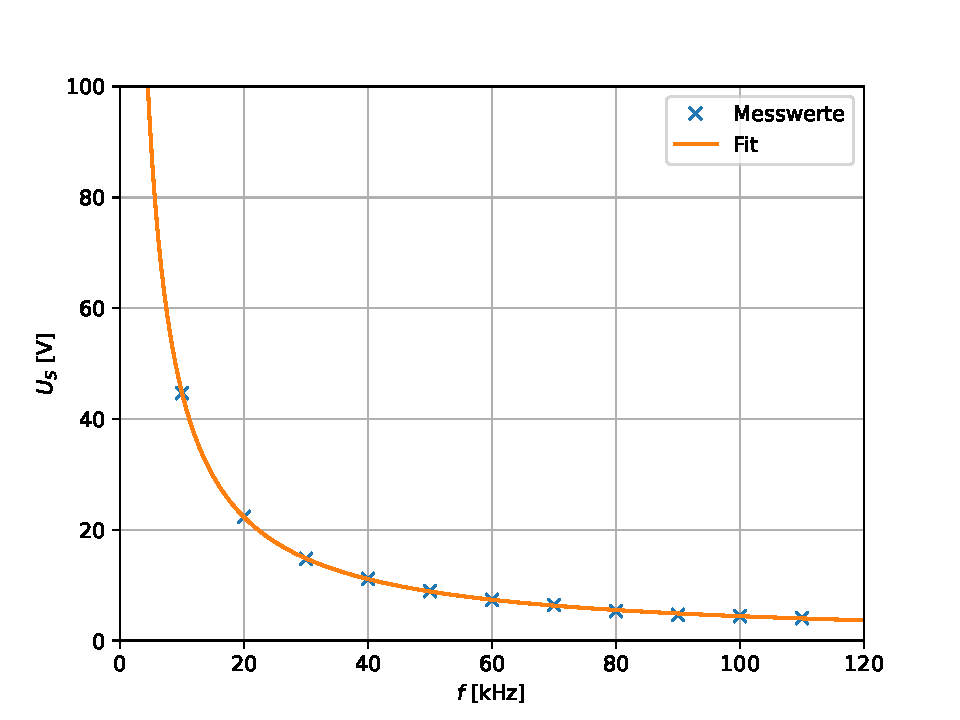
\includegraphics{plot1.pdf}
  \caption{Verlauf der Sägezahnspannung.}
  \label{fig:plot1}
\end{figure}

In Abbildung (\ref{fig:plot2}) ist die Fouriereihe der Dreiecksspannung zu erkennen. 
\begin{figure}[H]
  \centering
  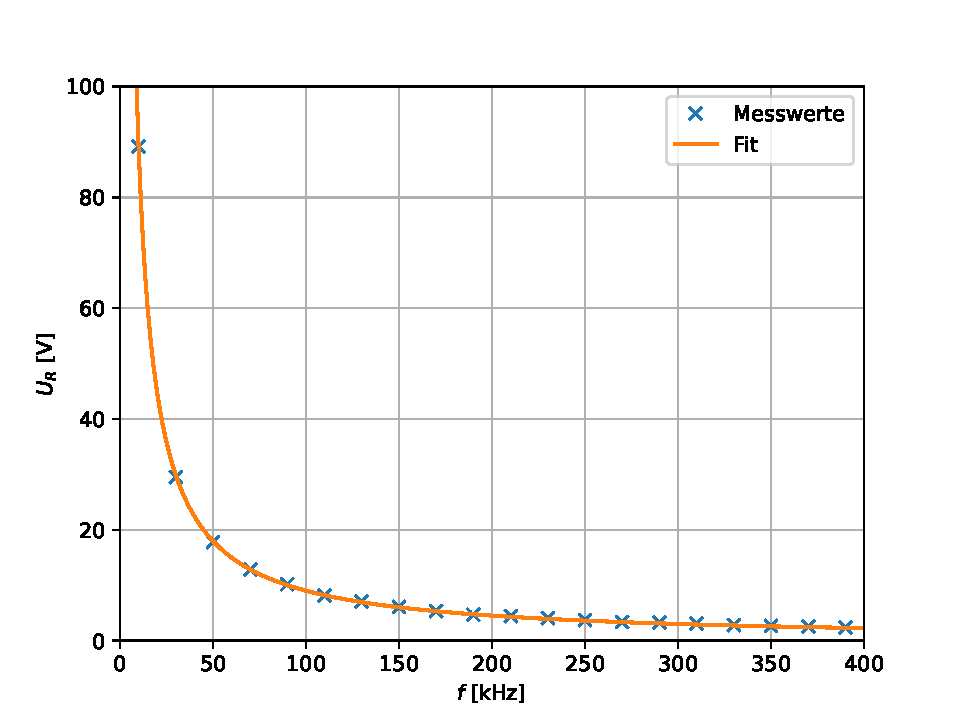
\includegraphics{plot2.pdf}
  \caption{Verlauf der Dreiecksspannung.}
  \label{fig:plot2}
\end{figure}

Außerdem ist in Abbildung (\ref{fig:plot3}) die Fouriereihe der 

\subsection{Fourieanalyse}



%Siehe \autoref{fig:plot}!